

% This file was created with tikzplotlib v0.10.1.
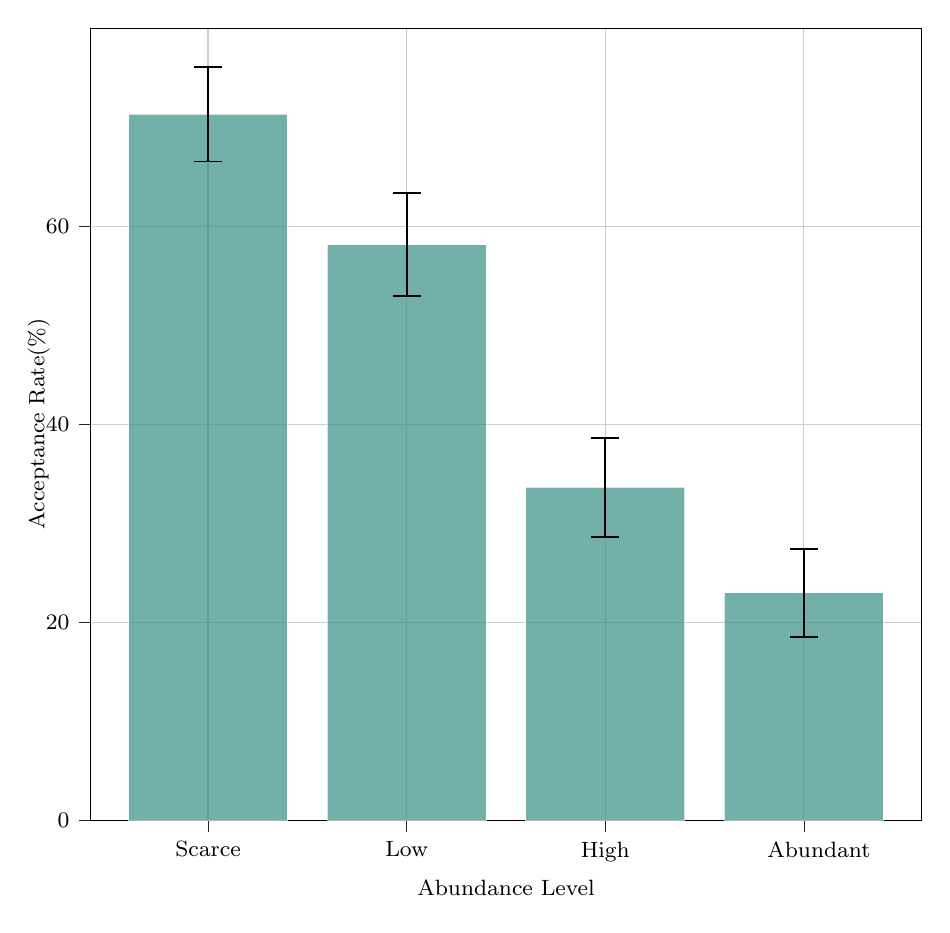
\begin{tikzpicture}

    \definecolor{darkslategrey38}{RGB}{38,38,38}
    \definecolor{darkslategrey66}{RGB}{66,66,66}
    \definecolor{lightgrey204}{RGB}{204,204,204}
    \definecolor{mediumseagreen56142132}{RGB}{56,142,132}
    
    \begin{axis}[
        width=1\textwidth,    % 设置宽度
        height=0.96\textwidth,  % 16:9比例
        axis line style={black},
        tick align=outside,     % 刻度线向外
        axis lines=box,         % 显示完整边框
        tick pos=left,          % y轴刻度线只在左侧
        xtick pos=bottom,       % x轴刻度线只在底部
        clip=true,              % 裁剪超出内容
        unbounded coords=jump,
        x grid style={lightgrey204},
        xlabel=Abundance Level,
        xlabel style={font=\footnotesize},
        xmajorticks=true,
        xmin=-0.59, xmax=3.59,
        xtick style={color=darkslategrey38},
        xtick={0,1,2,3},
        xticklabels={Scarce,Low,High,\hspace{8pt} Abundant},
        xticklabel style={font=\footnotesize,rotate=0},
       % xticklabel 4/.style={xshift=20pt, font=\scriptsize},
        y grid style={lightgrey204},
        ylabel=Acceptance Rate(\%),
        ylabel style={font=\footnotesize ,
            inner sep=0pt,    % 减少标签和轴的距离
            yshift=-5pt       % 微调标签位置
        },
        ymajorgrids,
        ytick={0,20,40,60},  % 添加y轴刻度
        yticklabel style={font=\footnotesize},
        ymin=0, ymax=80,
        ytick style={color=darkslategrey38},
        grid=major,
        grid style={lightgrey204},
        % yticklabel format={\pgfmathprintnumber{#1}},  % 格式化y轴标签
        every outer x axis line/.append style={black},
        every outer y axis line/.append style={black}
    ]
    
  \draw[draw=white,fill=mediumseagreen56142132,opacity=0.7] (axis cs:-0.4,0) rectangle (axis cs:0.4,71.304347826087);
\draw[draw=white,fill=mediumseagreen56142132,opacity=0.7] (axis cs:0.6,0) rectangle (axis cs:1.4,58.1395348837209);
\draw[draw=white,fill=mediumseagreen56142132,opacity=0.7] (axis cs:1.6,0) rectangle (axis cs:2.4,33.6231884057971);
\draw[draw=white,fill=mediumseagreen56142132,opacity=0.7] (axis cs:2.6,0) rectangle (axis cs:3.4,22.9651162790698);
\addplot [line width=0.9pt, darkslategrey66]
table {%
0 nan
0 nan
};
\addplot [line width=0.9pt, darkslategrey66]
table {%
1 nan
1 nan
};
\addplot [line width=0.9pt, darkslategrey66]
table {%
2 nan
2 nan
};
\addplot [line width=0.9pt, darkslategrey66]
table {%
3 nan
3 nan
};
\path [draw=black, semithick]
(axis cs:0,66.5311154292968)
--(axis cs:0,76.0775802228771);

\path [draw=black, semithick]
(axis cs:1,52.9262116653737)
--(axis cs:1,63.3528581020681);

\path [draw=black, semithick]
(axis cs:2,28.6380850776403)
--(axis cs:2,38.6082917339539);

\path [draw=black, semithick]
(axis cs:3,18.5202889931626)
--(axis cs:3,27.4099435649769);

\addplot [semithick, black, mark=-, mark size=5, mark options={solid}, only marks]
table {%
0 66.5311154292968
1 52.9262116653737
2 28.6380850776403
3 18.5202889931626
};
\addplot [semithick, black, mark=-, mark size=5, mark options={solid}, only marks]
table {%
0 76.0775802228771
1 63.3528581020681
2 38.6082917339539
3 27.4099435649769
};
    \end{axis}
    
\end{tikzpicture}
    